\documentclass[a4paper,twoside]{article}
% Official class, fonts, layout and bibliography style are used unchanged.
\usepackage{epsfig}
\usepackage{subcaption}
\usepackage{calc}
\usepackage{amssymb,amstext,amsmath,amsthm}
\usepackage{multicol}
\usepackage{pslatex}
\usepackage{apalike}
\usepackage{algorithm2e}
\usepackage[bottom]{footmisc}
\usepackage[T1]{fontenc}
\usepackage[utf8]{inputenc}
\usepackage{graphicx,booktabs,array,tabularx,url}
\usepackage{tikz}
\usetikzlibrary{arrows.meta,positioning}
\usepackage[hidelinks]{hyperref}
\usepackage{SCITEPRESS}
\newcolumntype{Y}{>{\raggedright\arraybackslash}X}
\newcommand{\bits}{\operatorname{bits}}
\newcommand{\rank}{\operatorname{rank}}
\newcommand{\aifootnote}{\footnote{Drafting used Codex \cite{codex}. See the disclosure.}}
\newlength{\pubtablewidth}
\setlength{\pubtablewidth}{\textwidth}


\hypersetup{pdftitle={Companion Evidence for Exact Bidirectional Steganographic Transport},pdfauthor={},pdfsubject={Anonymous companion artifact; supplementary submission status unconfirmed}}
\renewcommand{\thefigure}{S\arabic{figure}}
\renewcommand{\thetable}{S\arabic{table}}
\renewcommand{\thesection}{S\arabic{section}}
\begin{document}
\title{Companion Evidence for Exact Bidirectional Steganographic Transport}
\author{}
\keywords{Artifact Recovery, Capacity, Detectability, Reproducibility.}
\abstract{This companion supplies retained artifact examples, expanded numerical tables, development serialization comparisons, arithmetic diagnostics and reproducibility details for the main paper. It adds no experiment, model inference, hypothesis test or independent sample. Prospective held-out results, development qualification, repeated development GPU timings and repeated context scores are kept separate. The main paper contains the protocol, principal outcomes and central limitations and does not depend on this companion being reviewed. A separate supplementary upload for an ICAART regular paper has not been verified in the official instructions. This document is therefore prepared as a companion artifact, not represented as accepted supplementary submission material.}
\onecolumn\maketitle\normalsize\setcounter{footnote}{0}\vfill

\section{\uppercase{Retained Bidirectional Examples}}
Figure~\ref{fig:examples} uses the first manifest-ordered fixed-rank held-out example in each direction. Selection was determined before appearance was inspected. The full text carrier contains 616 tokens. Its displayed excerpt is literal, with line wrapping only. Complete example files accompany the manuscript under \texttt{examples/}; their hashes and original evidence locations are recorded in the accompanying index. The compilation-only source ZIP contains their figure export. They contain public development or held-out source material, not an encryption key or the shared RGB row. Drafting assistance throughout this companion is disclosed at its end \cite{codex}.

\begin{figure*}[!t]
\centering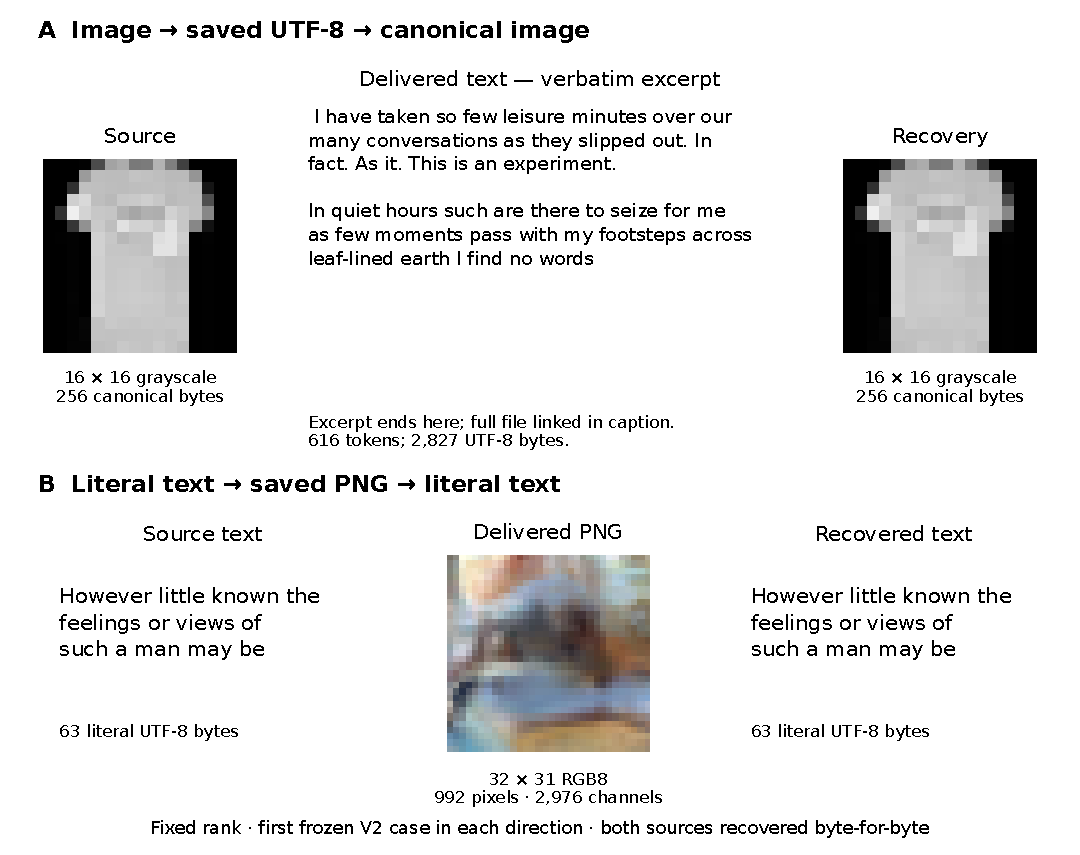
\includegraphics[width=\textwidth]{figures/figure1_transport.pdf}
\caption{Actual source, delivered carrier and recovery for the first fixed-rank held-out group in each direction. The top row transports a canonical $16\times16$ grayscale array, exactly 256 raw pixel bytes, through saved UTF-8. Its carrier excerpt is explicitly incomplete and is not rewritten. Full UTF-8 accompanies the draft at \texttt{examples/HI1-prompt1-fixed/carrier.txt}. The bottom row transports all 63 literal UTF-8 bytes through the shown $32\times31$ RGB PNG. Real pixels are enlarged with nearest-neighbor interpolation and preserved aspect ratio. Fresh receivers use only their own carrier, model/profile, shared context and key. Source bytes remain evaluator-only. The withheld 96-byte context row completes an internal $32\times32$ model canvas. Exact image recovery concerns canonical pixels, not an arbitrary original image container.}
\label{fig:examples}
\end{figure*}

The source-image PNG is a view of the canonical payload. Comparing two viewable PNGs alone is not the evaluator's test. It separately checks all 256 recovered raw pixels. In the reverse direction the recovered text is compared byte for byte, including literal punctuation and any non-ASCII encoding. Neither successful decryption nor visual similarity substitutes for those equality checks.

\begin{figure*}[!t]
\centering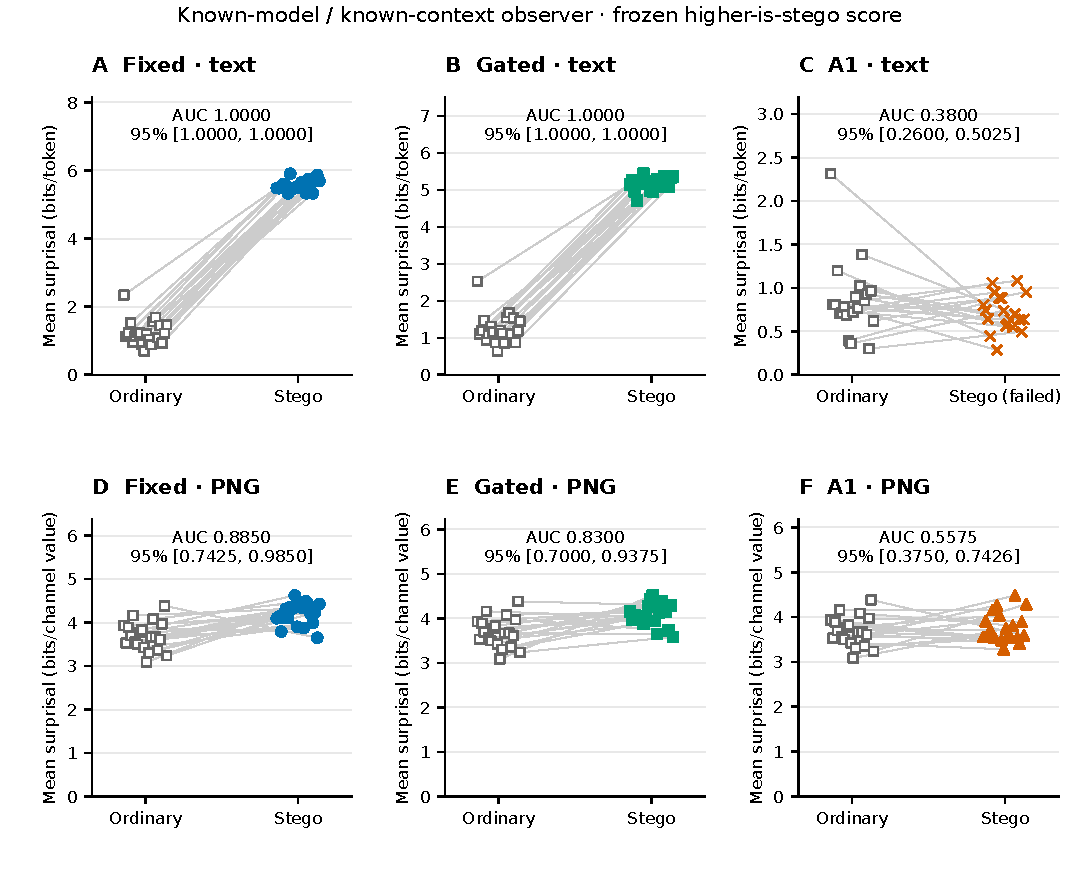
\includegraphics[width=\textwidth]{figures/figure3_detectability.pdf}
\caption{Whole-carrier mean-surprisal scores for the known-model, correct-context observer. Each panel shows 20 stego carriers and 20 matched ordinary observations with payload-group links. Failed A1 text carriers remain included. Text controls share prefixes of one trace per group, while PNG methods share full controls. Panel scales differ. AUC orientation is always higher-is-stego, with accepted 95\% grouped intervals. Complete empirical separation in the small fixed/gated text samples, including collapsed bootstrap intervals, does not establish perfect population detection.}
\label{fig:detectability-supp}
\end{figure*}

\section{\uppercase{Complete Prospective Tables}}
Table~\ref{tab:rates} preserves the six method/direction cells, rate intervals and original prospective timing. All 20 arithmetic-text failures remain in attempted counts and contribute zero exact goodput. Table~\ref{tab:detect-full} provides both frozen detector scores, including below-chance point estimates and failed delivered carriers. No observer orientation is reversed. The grouped intervals retain payload class or text-length strata and shared controls, as specified in the main paper.

\begin{table*}[!t]
\caption{Expanded prospective recovery, goodput and runtime. There are 20 payload groups in each cell. Recovery intervals use two-sided 95\% Clopper--Pearson bounds. Goodput intervals use 2,000 stratified payload-group bootstrap draws. Phase times and charged pair times are overlapping boundaries, not costs to add. Text goodput is bits/token and PNG goodput bits/channel value.}
\label{tab:rates}\centering\small
\setlength{\tabcolsep}{3pt}
\setlength{\pubtablewidth}{\dimexpr\linewidth-36pt\relax}
\begin{tabular}{@{}>{\raggedright\arraybackslash}p{0.130\pubtablewidth}>{\raggedright\arraybackslash}p{0.180\pubtablewidth}>{\raggedright\arraybackslash}p{0.210\pubtablewidth}>{\raggedright\arraybackslash}p{0.105\pubtablewidth}>{\raggedright\arraybackslash}p{0.105\pubtablewidth}>{\raggedright\arraybackslash}p{0.120\pubtablewidth}>{\raggedright\arraybackslash}p{0.150\pubtablewidth}@{}}
\toprule
Carrier / method & Exact / attempted; 95\% interval & Exact goodput; 95\% interval & Encode phase (s) & Decode phase (s) & Charged pair (s) & Failure \\
\midrule
UTF-8 / Fixed & 20/20\newline [83.16, 100.00]\% & 3.3247\newline [3.3247, 3.3247] & 45.63 & 45.31 & 123.33 & None \\[4pt]
UTF-8 / Gated & 20/20\newline [83.16, 100.00]\% & 3.1246\newline [3.1054, 3.1441] & 57.31 & 57.30 & 147.29 & None \\[4pt]
UTF-8 / A1 & 0/20\newline [0.00, 16.84]\% & 0.0000\newline [0.0000, 0.0000] & 398.15 & 396.01 & 826.57 & Token-cap capacity \\[4pt]
PNG / Fixed & 20/20\newline [83.16, 100.00]\% & 0.2505\newline [0.2473, 0.2535] & 85.27 & 85.31 & 178.18 & None \\[4pt]
PNG / Gated & 20/20\newline [83.16, 100.00]\% & 0.2505\newline [0.2473, 0.2535] & 85.29 & 85.65 & 178.53 & None \\[4pt]
PNG / A1 & 20/20\newline [83.16, 100.00]\% & 0.2505\newline [0.2473, 0.2535] & 85.59 & 85.77 & 179.01 & None \\[4pt]
\bottomrule
\end{tabular}

\end{table*}

\begin{table*}[!t]
\caption{Full exploratory correct-context detection. Scores are whole-carrier mean surprisal and mean $\log_2$ rank, with higher always indicating stego. Intervals are the accepted 95\% grouped percentiles. Each row has 20 scorable stego files and 20 matched ordinary artifacts. These associations use only 40 independent ordinary traces across the two directions, not 120 controls or 240 score observations. All 20 failed arithmetic text carriers are included. No duplicates or unscorable artifacts were dropped. A collapsed empirical interval does not establish perfect population detection.}
\label{tab:detect-full}\centering\small
\setlength{\tabcolsep}{3pt}
\setlength{\pubtablewidth}{\dimexpr\linewidth-30pt\relax}
\begin{tabular}{@{}>{\raggedright\arraybackslash}p{0.160\pubtablewidth}>{\raggedright\arraybackslash}p{0.200\pubtablewidth}>{\raggedright\arraybackslash}p{0.250\pubtablewidth}>{\raggedright\arraybackslash}p{0.120\pubtablewidth}>{\raggedright\arraybackslash}p{0.145\pubtablewidth}>{\raggedright\arraybackslash}p{0.125\pubtablewidth}@{}}
\toprule
Carrier / method & Frozen score & AUC [grouped 95\% interval] & Scorable stego & Unique matched controls & Failed stego included \\
\midrule
UTF-8 / Fixed & Mean surprisal & 1.0000 [1.0000, 1.0000] & 20 & 20 & 0 \\[4pt]
UTF-8 / Fixed & Mean log2 rank & 1.0000 [1.0000, 1.0000] & 20 & 20 & 0 \\[4pt]
UTF-8 / Gated & Mean surprisal & 1.0000 [1.0000, 1.0000] & 20 & 20 & 0 \\[4pt]
UTF-8 / Gated & Mean log2 rank & 1.0000 [1.0000, 1.0000] & 20 & 20 & 0 \\[4pt]
UTF-8 / A1 & Mean surprisal & 0.3800 [0.2600, 0.5025] & 20 & 20 & 20 \\[4pt]
UTF-8 / A1 & Mean log2 rank & 0.3600 [0.2425, 0.4801] & 20 & 20 & 20 \\[4pt]
PNG / Fixed & Mean surprisal & 0.8850 [0.7425, 0.9850] & 20 & 20 & 0 \\[4pt]
PNG / Fixed & Mean log2 rank & 0.8400 [0.6825, 0.9650] & 20 & 20 & 0 \\[4pt]
PNG / Gated & Mean surprisal & 0.8300 [0.7000, 0.9375] & 20 & 20 & 0 \\[4pt]
PNG / Gated & Mean log2 rank & 0.7700 [0.6299, 0.8975] & 20 & 20 & 0 \\[4pt]
PNG / A1 & Mean surprisal & 0.5575 [0.3750, 0.7426] & 20 & 20 & 0 \\[4pt]
PNG / A1 & Mean log2 rank & 0.5750 [0.4050, 0.7576] & 20 & 20 & 0 \\[4pt]
\bottomrule
\end{tabular}

\end{table*}

The exact-goodput difference between gated and fixed text is $-0.2000$ bits/token [$-0.2192$, $-0.1805$]. The corresponding charged-time difference is 23.96 seconds [20.34, 27.58]. For PNG, gated minus fixed charged time is 0.35 seconds [$-0.21$, 0.98]; arithmetic minus fixed is 0.83 seconds [0.38, 1.25]. All three PNG goodputs are identical by this allocation's fixed carrier size and exact recovery. The paired arithmetic-minus-fixed PNG mean-surprisal difference is $-0.4216$ bits/channel [$-0.5470$, $-0.3008$]. These are retained accepted comparisons, not post hoc selections of tests. The full machine-readable paired table is carried in \texttt{data/accepted\_paired\_differences.json}.

For equal all-success binary cells, the observed difference is zero but the conservative paired recovery bound remains $\pm19.68$ percentage points. It derives from the frozen 97.5\% marginal Clopper--Pearson bounds. This prevents the zero-width paired bootstrap display from being interpreted as a population equivalence statement. The sample remains 20 allocated groups per direction.

\section{\uppercase{Packet and Capacity Accounting}}
The packet consists of a 12-byte nonce, 264 encrypted bytes and a 16-byte tag. Its eight-byte protected header records version, kind, length and dimensions. The 256-byte slot is full for images, but has a mean 162.8 padding bytes for held-out texts. Thus 36 framing/encryption bytes and slot padding are separate costs. Fixed radix 16 requires no rank-alignment padding. The accompanying protocol identity record retains the exact framing identifier and unrounded entropy thresholds.

\begin{figure*}[!t]
\centering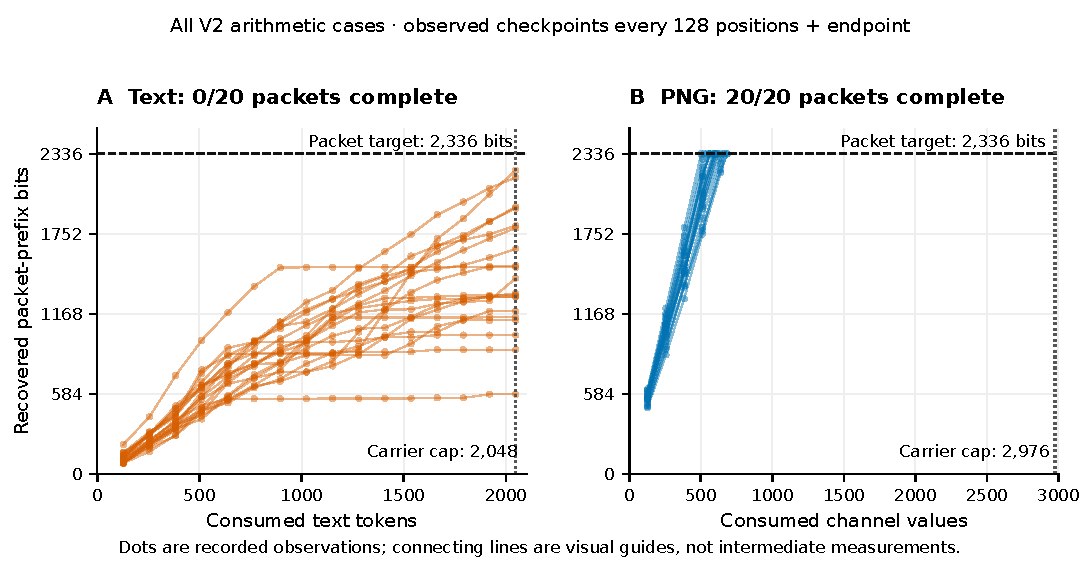
\includegraphics[width=\textwidth]{figures/figureS1_arithmetic_capacity.pdf}
\caption{Arithmetic packet-prefix accumulation for all 20 prospective text and 20 PNG cases. Dots are retained observations every 128 consumed symbols and at the final endpoint. Connecting lines are visual guides, not unrecorded intermediate measurements. The target is 2,336 useful packet bits. Text reaches its 2,048-token cap with only 581--2,216 bits. PNG reaches the target before ordinary completion fills the remaining canvas. Curves stop at the packet endpoint and do not include emitted zero suffix bits as useful information. Carrier units differ between panels. Isolated unchanged intervals in two failed texts and one successful PNG do not establish sustained stagnation as the text-failure cause.}
\label{fig:arithmetic}
\end{figure*}

\begin{table*}[!t]
\caption{Overhead means for every prospective method/direction cell. The packet's 36 framing bytes and slot padding are separate. A1 packet-positive and zero-bit positions partition its packet span. Its termination position overlaps the last positive position and is not added again. Emitted zero suffix and lookahead-zero diagnostics also overlap conceptually and are not extra payload. Text A1 has no complete-packet transport rate. The fixed full PNG has 2,976 channels. Serialized expansion divides delivered file bytes by canonical source bytes.}
\label{tab:overhead}\centering\small
\setlength{\tabcolsep}{3pt}
\setlength{\pubtablewidth}{\dimexpr\linewidth-54pt\relax}
\begin{tabular}{@{}>{\raggedright\arraybackslash}p{0.140\pubtablewidth}>{\raggedright\arraybackslash}p{0.100\pubtablewidth}>{\raggedright\arraybackslash}p{0.160\pubtablewidth}>{\raggedright\arraybackslash}p{0.120\pubtablewidth}>{\raggedright\arraybackslash}p{0.120\pubtablewidth}>{\raggedright\arraybackslash}p{0.130\pubtablewidth}>{\raggedright\arraybackslash}p{0.140\pubtablewidth}>{\raggedright\arraybackslash}p{0.090\pubtablewidth}@{}}
\toprule
Carrier / method & Slot pad (B) & Packet-positive positions & Skipped positions & Zero-bit positions & Completion positions & Packet bits / span symbol & Suffix bits \\
\midrule
UTF-8 / Fixed & 0.0 & 584.00 & 0.00 & 0.00 & 32.00 & 4.000 & 0.0 \\[4pt]
UTF-8 / Gated & 0.0 & 584.00 & 39.80 & 0.00 & 32.00 & 3.747 & 0.0 \\[4pt]
UTF-8 / A1 & 0.0 & 399.40 & 0.00 & 1648.60 & 0.00 & --- & 0.0 \\[4pt]
PNG / Fixed & 162.8 & 584.00 & 0.00 & 0.00 & 2392.00 & 4.000 & 0.0 \\[4pt]
PNG / Gated & 162.8 & 584.00 & 100.50 & 0.00 & 2291.50 & 3.451 & 0.0 \\[4pt]
PNG / A1 & 162.8 & 508.20 & 0.00 & 89.65 & 2378.15 & 3.934 & 28.9 \\[4pt]
\bottomrule
\end{tabular}

\end{table*}

\subsection{A1 Interval Rules and Diagnostic Limits}
The A1 implementation uses 32-bit half-open intervals. After selecting a subinterval $[l,u)$, its common-prefix length is
\begin{equation}
b=32-\operatorname{bitlength}\bigl(l\mathbin{\mathrm{xor}}(u-1)\bigr).
\end{equation}
It emits the first $b$ bits of $l$. With $M=2^{32}-1$, the next interval is
\begin{align}
l'&=(l\ll b)\mathbin{\&}M,\\
u'&=\bigl(((u-1)\ll b)\mathbin{\&}M\bigr)+2^b,
\end{align}
where the mask applies before the final addition in the expression for $u'$. The main paper gives the exact partitioning and zero-extension rules. Unlike a general arithmetic coder with an additional underflow-renormalization mechanism, this adaptation does not add an E3 rule or a final endpoint dump. The inspected Ziegler reference \cite{ziegler} is algorithmic attribution; its source was not copied because a reuse license was not identified.

A concrete independently checked limitation is a narrow interval straddling a leading-bit boundary whose quantized distribution retains only one nonzero bin. Selecting that bin can leave the interval unchanged indefinitely. This is a property of the frozen adaptation, not proof that every zero-bit step stagnates. In the actual prospective text cases, final recovered information closely tracks accumulated eligible surprisal. Two cases have one and three isolated unchanged steps, with no consecutive run beyond one. A successful PNG also has one isolated step. The 40 retained prospective audits agree with the independent partition/interval oracle and source-prefix checks. No arithmetic text case reaches finite-message zero-extension or termination, so its failure is not evidence of a termination bug.

Detailed packet windows and rank traces remain private. The retained public endpoint and 128-position checkpoint summaries are sufficient to inspect capacity without exposing those private audit streams. Complete packet-prefix bits are capped at 2,336 for successful PNGs, with suffix diagnostics reported separately. No line between observed checkpoints is used to infer a missing trace value.

\section{\uppercase{Development Serialization Evidence}}
\begin{figure*}[!t]
\centering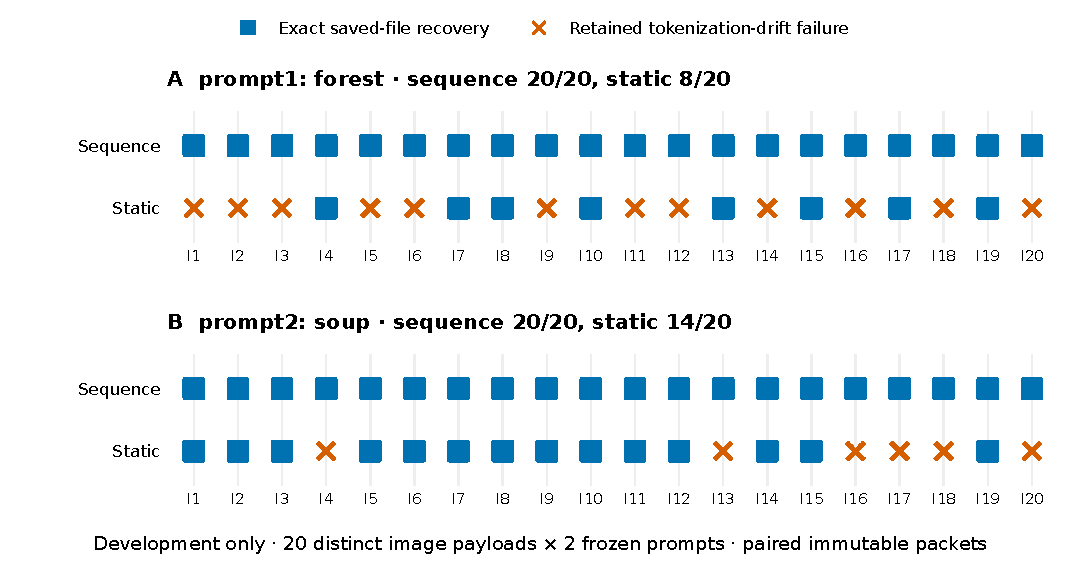
\includegraphics[width=\textwidth]{figures/figureS2_text_consistency.pdf}
\caption{Paired development comparison of saved-text consistency, separate from the prospective study. Each column is one of 20 distinct image payloads under both frozen prompts. Sequence filtering checks the complete carrier prefix; static filtering checks singleton tokens only. Other candidate, probability, coding and completion rules are held fixed. Each context-specific pair uses the same sealed packet. Sequence recovery is 20/20 under each prompt. Static recovery is 8/20 for the forest prompt and 14/20 for the soup prompt, with 18 retained drift/replay failures. Static text is neither repaired nor accompanied by sender identifiers. The 40 context-specific cases are not 40 independent payloads.}
\label{fig:consistency}
\end{figure*}

The second prompt is ``Explain how a home cook prepares a simple vegetable soup. Use continuous prose.'' It was frozen before its carriers were generated. The singleton arm lazily caches eligibility for encountered candidates but does not use the complete-prefix assertion. A final mismatch therefore remains a saved artifact and experimental outcome. The main sequence arm retains strict final consistency. This comparison adapts an existing singleton mask and published stepwise verification \cite{rankcloak,consistency}; it does not introduce a new tokenization theory.

Development qualification accounts for 152 stego outcomes. Fixed sequence text and fixed PNG each recover 40/40. Gated coding recovers 8/8 in each direction. A1 PNG recovers 8/8, while A1 text retains eight capacity failures. Static text recovers 22/40. Sixteen ordinary traces and 48 controls are accounted for. One historical static matched-control prefix was unavailable and remains unscored, not silently regenerated. These experiments establish configuration qualification and serialization behavior, not an expanded held-out sample.

Twenty predetermined fixed PNG development carriers, covering both shared rows, were re-saved with another lossless compression setting and no ancillary metadata. Dimensions, RGB mode and every pixel byte remained equal. Fresh receivers then recovered all 20 original payloads exactly. These are preservation checks of existing carriers, not independent new transmissions. Text files also passed raw UTF-8 byte save/load checks. Ordinary CPU verification supports packet bounds, wrong-key authentication failure, nibble inversion, UTF-8 consistency, conditional RGB probabilities and separately written arithmetic oracles. Routine test counts remain in the supporting evidence rather than scientific outcome tables.

\section{\uppercase{Context Scores and Descriptive Shifts}}
Table~\ref{tab:png-context-scores} expands the main context figure with both scores and paired intervals. The same 80 PNGs are rescored, and each of 20 controls is shared across methods. Twenty length-stratified payload groups, not 60 independent pairs, are resampled jointly with both observer conditions. The fixed primary decrease is supported by an interval below zero. Gated and A1 changes remain uncertain. A resolved change in one cell and an unresolved change in another do not establish a between-method interaction.

\begin{table*}[!t]
\caption{Correct and mismatched PNG AUCs for both frozen scores. Each row contains 20 scorable stego PNGs and 20 unique matched controls. Values and paired 95\% intervals are the accepted 2,000-draw length-stratified group analysis, with conditions, methods and shared controls kept together. Higher score always indicates stego. The paired interval is computed from within-draw differences, not by subtracting marginal interval endpoints. There are no failed scores or exclusions.}
\label{tab:png-context-scores}\centering\small
\begin{tabular}{@{}llccc@{}}
\toprule
Method & Score & Row1 AUC [95\% CI] & Row2 AUC [95\% CI] & Change [95\% CI] \\
\midrule
Fixed & Surprisal & 0.8850 [0.7425, 0.9850] & 0.6975 [0.5150, 0.8700] & -0.1875 [-0.2775, -0.1000] \\
Fixed & $\log_2$ rank & 0.8400 [0.6825, 0.9650] & 0.6625 [0.4725, 0.8475] & -0.1775 [-0.2800, -0.0950] \\
Gated & Surprisal & 0.8300 [0.7000, 0.9375] & 0.7475 [0.6074, 0.8825] & -0.0825 [-0.1625, 0.0100] \\
Gated & $\log_2$ rank & 0.7700 [0.6299, 0.8975] & 0.7225 [0.5775, 0.8675] & -0.0475 [-0.1301, 0.0375] \\
A1 & Surprisal & 0.5575 [0.3750, 0.7426] & 0.5925 [0.4124, 0.7725] & +0.0350 [-0.0225, 0.1050] \\
A1 & $\log_2$ rank & 0.5750 [0.4050, 0.7576] & 0.5975 [0.4175, 0.7726] & +0.0225 [-0.0325, 0.0725] \\
\bottomrule
\end{tabular}

\end{table*}

\begin{figure*}[!t]
\centering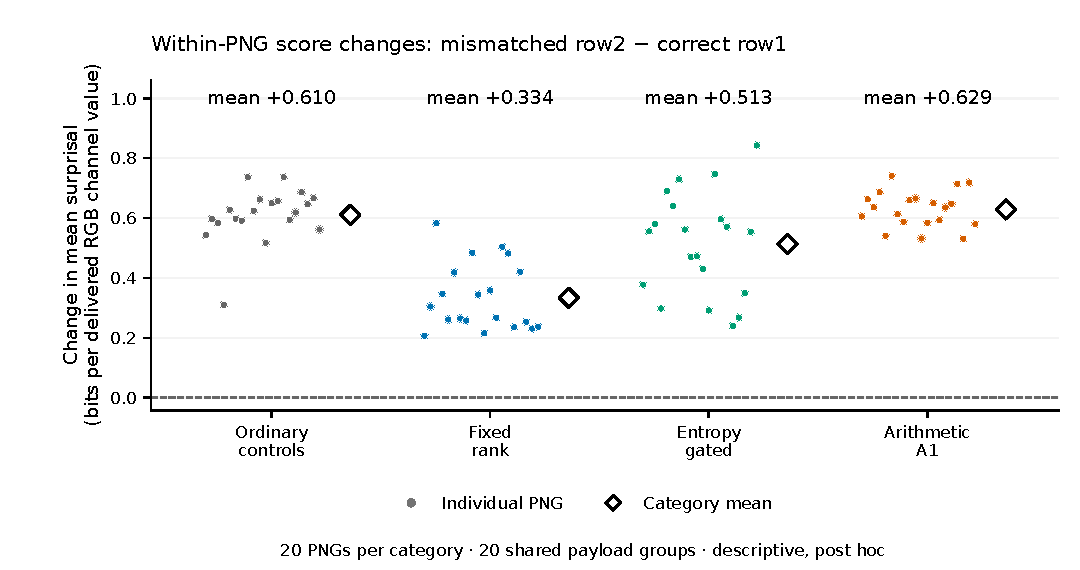
\includegraphics[width=\textwidth]{figures/score_shifts.pdf}
\caption{Descriptive within-PNG score shifts, row2 minus row1, in bits per delivered RGB channel value, not changes in AUC. All 80 observations come from the retained context study, 20 per category, with the same 20 payload groups and shared controls. Deterministic horizontal offsets only separate points. Open diamonds and annotations are category means. Row2 is the previously frozen random-RGB row, whereas row1 comes from a generated image. This post hoc analysis adds no test, interval or transmission. Mean shifts show score movement, while AUC depends on the full rankings. The plot does not establish secrecy or isolate a causal mechanism.}
\label{fig:png-score-shifts}
\end{figure*}

\begin{table*}[!t]
\caption{Descriptive score means and within-artifact changes for Figure~\ref{fig:png-score-shifts}. Each category contains 20 observations. Units are bits per delivered RGB channel value. Controls are counted once, and the four categories share 20 groups. These are post hoc summaries without added inferential claims.}
\label{tab:score-shifts}\centering\small
\begin{tabular}{@{}lrrrrr@{}}
\toprule
Category & Count & Row1 mean & Row2 mean & Mean change & Median change \\
\midrule
Ordinary controls & 20 & 3.683649 & 4.294085 & +0.610436 & +0.621412 \\
Fixed rank & 20 & 4.191273 & 4.525204 & +0.333930 & +0.285979 \\
Entropy gated & 20 & 4.074328 & 4.587583 & +0.513255 & +0.554706 \\
Arithmetic A1 & 20 & 3.769649 & 4.398864 & +0.629215 & +0.635652 \\
\bottomrule
\end{tabular}

\end{table*}

The paired fixed-minus-control mean score gap decreases from 0.507624 to 0.231119, a change of $-0.276505$ bits per channel. Controls have a larger mean score increase than fixed carriers, consistent with this narrower gap. The pattern does not establish an independently confirmed mechanism for the AUC difference. It cannot separate context correctness from differences between generated-image row statistics and random RGB statistics. Near-chance AUC also does not establish cryptographic secrecy or broad resistance to detection.

\section{\uppercase{Complete GPU Benchmark}}
\begin{table*}[!t]
\caption{All five development payload/method combinations. Latencies are means of charged fresh-process encode/decode times. Fixed has three timing repetitions per payload; gating and A1 have one comparison on the 32-byte payload. Speedups are ratios of matched mean pair times. Per-row throughput is the accepted mean of individual source-bytes/pair-second ratios; the main headline instead pools bytes and times over nine fixed comparisons. All 11 comparisons and 22 recoveries preserve exact stream, carrier and source-byte equality. Repetitions do not increase the independent payload count.}
\label{tab:benchmark}\centering\small
\setlength{\tabcolsep}{3pt}
\setlength{\pubtablewidth}{\dimexpr\linewidth-36pt\relax}
\begin{tabular}{@{}>{\raggedright\arraybackslash}p{0.140\pubtablewidth}>{\raggedright\arraybackslash}p{0.100\pubtablewidth}>{\raggedright\arraybackslash}p{0.180\pubtablewidth}>{\raggedright\arraybackslash}p{0.180\pubtablewidth}>{\raggedright\arraybackslash}p{0.100\pubtablewidth}>{\raggedright\arraybackslash}p{0.180\pubtablewidth}>{\raggedright\arraybackslash}p{0.120\pubtablewidth}@{}}
\toprule
Payload / method & Bytes / repeats & Reference encode / decode (s) & Graph encode / decode (s) & Pair speedup & Recovered B/s reference $\rightarrow$ graph & Equivalence \\
\midrule
T1 / Fixed & 32 / 3 & 88.97 / 89.28 & 17.38 / 17.28 & 5.14$\times$ & 0.180 $\rightarrow$ 0.923 & Exact \\[4pt]
T1 / Gated & 32 / 1 & 90.17 / 90.07 & 17.38 / 17.23 & 5.21$\times$ & 0.178 $\rightarrow$ 0.925 & Exact \\[4pt]
T1 / A1 & 32 / 1 & 91.83 / 91.03 & 17.83 / 17.28 & 5.21$\times$ & 0.175 $\rightarrow$ 0.911 & Exact \\[4pt]
T4 / Fixed & 96 / 3 & 89.12 / 89.09 & 17.34 / 17.29 & 5.15$\times$ & 0.539 $\rightarrow$ 2.772 & Exact \\[4pt]
T5 / Fixed & 128 / 3 & 88.76 / 88.24 & 17.36 / 17.27 & 5.11$\times$ & 0.723 $\rightarrow$ 3.696 & Exact \\[4pt]
\bottomrule
\end{tabular}

\end{table*}

The three payloads were selected by first numeric development identifier within the 32--64, 65--96 and 97--128-byte bands, giving 32, 96 and 128 bytes. The same retained packet is used in each matched reference/graph comparison. Figure 4 of the main paper shows all nine fixed timing repetitions. Table~\ref{tab:benchmark} adds the two single-payload methods. No parameter, context or seed sweep was performed.

Reference execution remains available and is the prospective baseline. The optional CUDA graph path uses static CUDA input/output buffers, three warmup forwards, capture of the unchanged network and synchronized replay. CPU normalization, mixture probabilities, rank ordering and serialization are identical. Exact stream digests include length-framed identifiers, float64 probabilities and rank order at every delivered channel. Their equality is stronger than accepting a numerical tolerance, but it is still evidence on the checked cases and stack, not a cross-platform theorem.

For the nine fixed comparisons, charged pair time averages 177.819 seconds reference and 34.642 seconds graph. Inside those totals, encode plus decode phases average 170.184 and 25.829 seconds, CUDA-event intervals 165.431 and 21.251 seconds, cold model loading 1.876 and 1.884 seconds, and graph setup zero and 1.174 seconds. The remaining charged time is approximately 5.758 and 5.755 seconds. CUDA intervals overlap the phases, and no component is charged a second time.

Peak allocated PyTorch memory is 484.479 versus 473.849 MiB. Peak reserved memory is 516 versus 744 MiB. Sampled process memory is 912 versus 1,176 MiB. These different views overlap. Process-specific \texttt{nvidia-smi pmon} observations use the child PID, with roughly 0.19-second polling. Driver windows, correlated samples and gaps prevent interpreting a single peak or sampled average as sustained utilization. All 45 benchmark model jobs, one short probe and 44 sender/receiver processes, have allocation and positive activity evidence. The probe is charged but not included in the matched timing means.

\section{\uppercase{Reproducibility and Evidence Boundaries}}
Checkpoint SHA-256 identities follow, wrapped without separators. Private paths, device serials and context bytes are omitted.
\begin{itemize}
\item Text GGUF SHA-256: \texttt{86c8ea6c8b755687d0b723176fcd0b24}\allowbreak\texttt{11ef80533d23e2a5030f845d13ab2db7}.
\item PixelCNN++ checkpoint SHA-256: \texttt{a5ed558f6d4098ce3cbfd47658b7e3be}\allowbreak\texttt{37fae77b71a90c8a56f46a6266ff833f}.
\end{itemize}
Text retains eight threads, a 4,096-token context, batch/microbatch one, full eligible-layer offload, all-position logits and context/KV reset between sequences. The image stack is Python 3.10.13, PyTorch 2.5.1+cu124, CUDA 12.4, cuDNN 90100, NumPy 2.2.6 and Pillow 12.3.0. Both use float64 probability bookkeeping. Disabled TF32/benchmarking, deterministic algorithms, synchronous launches and \texttt{CUBLAS\_WORKSPACE\_CONFIG=:4096:8} are retained. Text additionally disables llama.cpp graphs/fusion and retains its recorded float32 cuBLAS control.

Focused RankCloak adaptations use revision \texttt{ce853d4}. The PixelCNN++ port is \texttt{7cb4436}, with upstream \texttt{bbc1568}. Their notices are preserved. The checkpoint is \texttt{pcnn\_lr.0.00040\_}\allowbreak\texttt{nr-resnet5\_}\allowbreak\texttt{nr-filters160\_889.pth}, from the port author's linked distribution. Strict loading removes a uniform DataParallel prefix bijectively. No replacement model was trained.

Public verification checks saved hashes, complete allocation, source equality, profile identities and shared controls. It verifies recorded authentication, not a new private-key operation. Fresh neural reproduction requires pinned models, compatible GPU runtimes and original context/key/packet bindings. Source-containing review directories are evaluator inputs, never receiver inputs.

The accompanying numerical CSVs and manuscript index map every result to retained evidence. The compilation-only source ZIP needs standard TeX packages but no experimental repository, private runs, models or network.

\section*{\uppercase{AI Assistance Disclosure}}
OpenAI Codex assisted implementation, analysis/plotting scripts and drafting/editing \cite{codex}. Plots use retained observations, and examples are actual saved carriers. Manuscript preparation adds no experiment or substitute imagery. The authors remain responsible for verification and submission decisions.
\bibliographystyle{apalike}
{\small\bibliography{references}}
\end{document}








